\documentclass[12pt]{report}

\usepackage{mathptmx}
\usepackage{graphicx}
\usepackage{hyperref}
\usepackage{amsmath}
\usepackage{ amssymb }
\usepackage{setspace}
\usepackage{booktabs}
\usepackage{rotating}
\usepackage{makecell}
\usepackage{subcaption}

\usepackage{xcolor}
\hypersetup{
    colorlinks,
    linkcolor={red!50!black},
    citecolor={purple!50!black},
    urlcolor={blue!80!black}
}

\usepackage{titlesec}
\titleformat{\chapter}[hang]
{\bfseries\Huge}{\chaptertitlename\ \thechapter:}{16pt}{\Huge}
\titleformat{\section}
  {\Large\bfseries}{\thesection}{14pt}{}
\titleformat{\subsection}
  {\large\bfseries}{\thesubsection}{11pt}{}
  
  
\usepackage[font=small,labelfont=bf,textfont=bf]{caption}
%\newcommand{\cchapter}[1]{\chapter[#1]{\centering #1}}
\usepackage[top=1.0in,bottom=1.0in,left=1.0in,right=1.0in]{geometry} 

\usepackage{pdfpages}

\begin{document}
\includepdf[pages={1}]{certi.pdf}

\begin{spacing}{1.5}
\chapter{Introduction}

% NN has become defacto standard for NLP models
Machine Learning based methods have become a de facto standard for solving majority of Natural Language Processing problems. 
With the increase in complexity of models, it has become difficult to test and debug to see if they are robust for deployment.
The standard metrics for model evaluation are measured by averaging error over a testing dataset which is kept separate from training data.
While these metrics, like accuracy, are useful, developers can overestimate their models generalization capabilites as testing data is obtained in same manner like training data.
A  model can show impressive perfomance over these metrics, but it might be due to superficial cues which happens to be predictive most of the time \cite{jia2019}.

Recent research has shown that Complex models for Natural Language Processing are prone to ``brittleness'' i.e. ``different ways of phrasing the same sentence can often cause the model to output different predictions'' \cite{riberio2018}.
Moreover, NLP models are vulnerable to small changes in input \textit{(oversenstivity)}, called Adversarial pertrubations, which leads them to produce wrong output \cite{liang2018}.
The changes are small enough that it appears as same sentence semtanically (also syntactically in some case) to a human but causes ML model to mispredict.

In real world scenario, adversarial examples can be used to evaluate if deeper, intelligent patterns are recognized by the model so that it generalizes well and is robust.
Using these attacks, we can understand our model's capabilities and limitations, and, as a longstanding problem in AI, check true language understanding and reasoning abilities.
In addition, since an adversarial attack changes the output of a model, it poses security concerns. It can be used to exploit the model, for example, a spammer can generate adversarial pertrubations to evade a spam filter or evade a False news detector.
Hence, our objective for adversarial attacks is twofold: \textit{model evaluation and interpretation}, and \textit{exposing system vulnerability}.

There are several ways to generate adversarial examples but we are interested in \textbf{Universal Adversarial Triggers} that can be applied on any input sequence in the domain.
These are input independent sequence of tokens, which, when concatenated with input text, fools NLP models to mispredict. Since these tokens are input-agnostic, they pose a bigger threat than input-specific pertrubations, as they can be distributed to a large number and they work on majority of inputs. Additionally, global model behaviour insights can be drawn upon by universal triggers \cite{wallace2019}. In this project, we try to generate universal adversarial triggers for Text Classification NLP task as done in \cite{wallace2019, behjati2019}.
% about UNiversal triggers

\section{Text Classification}
Text Classification is a categorization problem in which a text, sentence, or document is assigned a predefined tag according to its content. It is one of the fundamental problems in Natural Language Processing which can be solved with various techniques like \textit{knowledge based methods, statical methods}, and other hybrid techniques.
Some real world examples of Text classification includes:
\begin{enumerate}
\item Spam Filters
\item Categorizing News articles and movie genre
\item Sentiment analysis or Opinion mining
\end{enumerate}
We demonstrate the effectiveness of adversarial examples using \textbf{Sentiment Analysis} classifier.

\section{Adversarial examples}
% Show CV example maybe

Adversarial example for text classification can be formally defined as follows:
Consider $f$ as a classifier function which classifies input $s \in S$ to one of the class $c \in C$, then $s'$ is an adversarial example if $s'$ is recognized in the same class $c$ by a Human observer, but $f(s) \neq f(s')$.

\subsection{Choice of adversarial examples: Granularity}
To generate adversarial example, we need a small ``change'' than can transform $s$ to $s'$. This change, in case of NLP, can be at following levels or granularity: \textit{character, words} and \textit{ sentence}.
\paragraph{Character Level}
At this granularity, the aim is to change characters of a word in order to generate small difference to have adversarial effect. Characters could be removed, added, or replaced to produce the change.
% TODO Add pros and cons
Fig. \ref{ebrahimi_word} shows character level changes that causes misclassification.
\begin{figure}[!h]
  \centering
  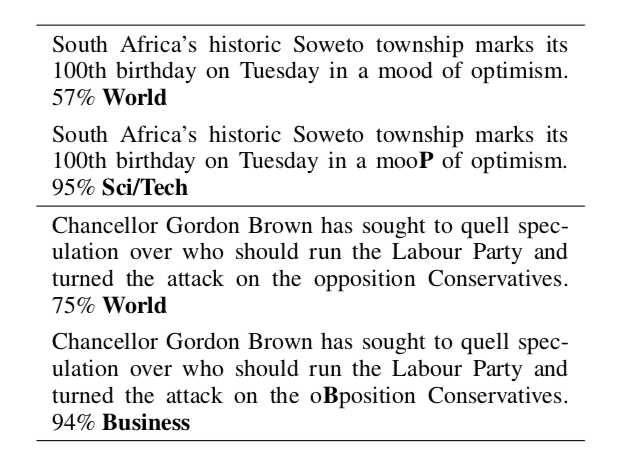
\includegraphics[width=0.5\linewidth]{./img/ebrahimi_char.png}
  \caption{Character level change \cite{ebrahimi2018}}
  \label{ebrahimi_word}
\end{figure}

\paragraph{Word Level}
At this granularity, the aim is to replace a word with a similar word to generate adversarial example. New words can also be added or existing words can be removed to bring the change.
% TODO add pros and cons
Fig. \ref{alzantot_senti} shows an word level adversarial example created by Alzantot et al. \cite{alzantot2018}.
\begin{figure}[!h]
  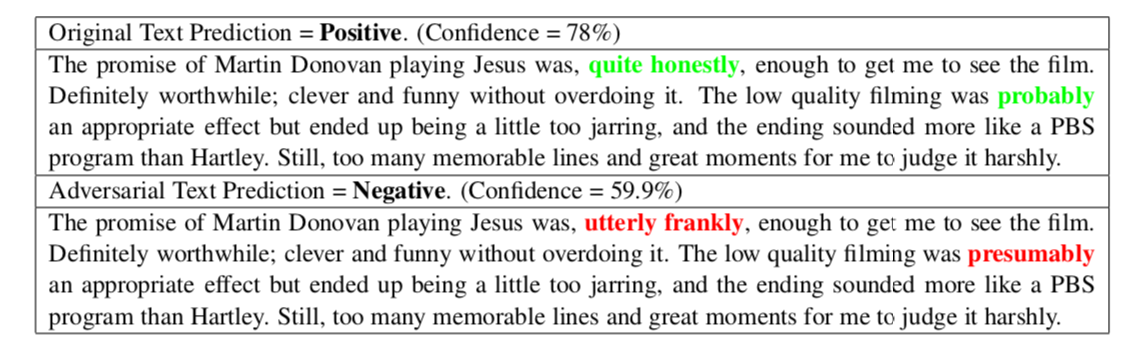
\includegraphics[width=\linewidth]{./img/alzantot_senti.png}
  \caption{Word level change \cite{alzantot2018}}
  \label{alzantot_senti}
\end{figure}

\paragraph{Senetence Level}
At this level, an adversarial example is created by paraphrasing the sentence, by removing a sentence, or by appending a new sentence, such that the meaning of the document remains the same as before.
% TODO add pros and cons
Fig. \ref{liang_sen} shows how addition of sentence causes model to misclassify text form \textit{Album} to \textit{Company}.

\begin{figure}[!h]
  \centering
  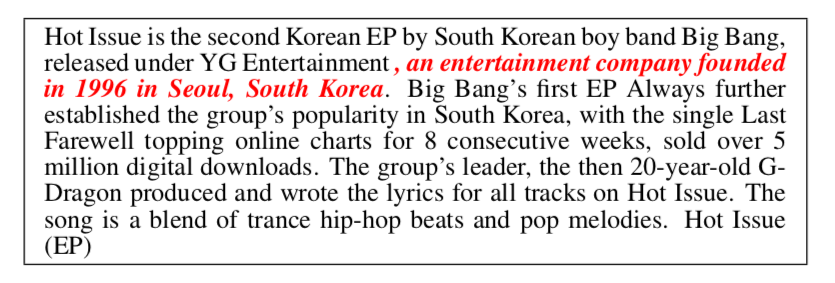
\includegraphics[width=0.8\linewidth]{./img/liang_sen.png}
  \caption{Sentence level change. 99.9\% \textit{Album} to 94.0\% \textit{Company} \cite{liang2018}}
  \label{liang_sen}
\end{figure}

\subsection{Universal Adversarial triggers}
\label{adv_theory}
Universal triggers poses highest form of adversarial threat for two reasons: (1) Access to target model is not required at target time (2) they decrease the barrier for an adversary. In addition, as noted by Moosavi-Dezfooli et al. \cite{moosavi-dezfooli}, universal triggers are often transferable accross models. Hence, an adversary might not need White-box, or gradients, access to a model and can even attack black-box targets.
Moreover, universal triggers are unique evaluation tools as they reveal general input-output patterns learnt by the model. This is used to learn about the biases learnt from the dataset.
\par
In Universal Adversarial triggers, we search for pertrubations at word level.
We try to find input-agnostic words that can be inserted in original sentence.
More specifically, we want a sequence of words $w$ that can be concatenated to input $s$ belonging to probablity distribution $P(L)$ that causes classifer $f$ to mispredict.
Hence, our adversarial example $s'$ will be of the form:
\begin{equation}
  \label{adv_s}
  s' = w \oplus s = s_i...s_k | w_1...w_m | s_{k+1}...s_j; \; (i,j) \in [0, len(s)] 
\end{equation}

To get the value of $w$, we maximize the classifier loss over all dataset. If true output is $y$, then the optimization needed to be solved is,
\begin{equation}
  \label{eq: optim}
  \hat{w} = \underset{w}{argmax} \; \mathcal{E}_{s \sim P(L)}[\mathcal{L}(y, f(s'))]
\end{equation}
Since we are optimizing the expected loss with respect to the
data distribution, the resulting sequence $\hat{w}$ would ideally be
universal. We constrain equation \ref{adv_s} to insert adversarial triggers at the beginning of the sentence. Hence, our $s'$ becomes:
\begin{equation}
  \label{eq: trigger}
  s' = w \oplus s = w_1...w_m \cdot s_1...s_n
\end{equation}

\paragraph{Problem statement}
We seek to find Universal Adversarial triggers $w$ that when appended to \ref{eq: trigger} will cause $f$ to misclassify. This problem is solved by finding solution $\hat{w}$ of equation \ref{eq: optim}. Through this adversarial attack, we check the robustness of the system as well as check the scope of bias and noise leading to oversensitivity to input.

% TODO write WHITE box is required

\chapter{Process Flow Diagram}
 The project can be logically divided into two modules - \textit{Classifier} and \textit{Generator}. \textit{Classifer} calculates the categorical class of the input text, while \textit{Generator} is used to generate adversarial triggers for this classifier. \textit{Generator} requires the \textit{gradients} of the \textit{Classifier} as we employ White-box attack on it. Top level process flow is shown in Fig \ref{img: top_level}.

Ideally, triggers should be stealthy enough that they should fool humans and they should not be too obvious - like ``best'' when targeting negative example.
However, the latter situation can be made stealthy by injecting triggers inbetween the words rather than at end points.

\begin{figure}[!h]
  \centering
  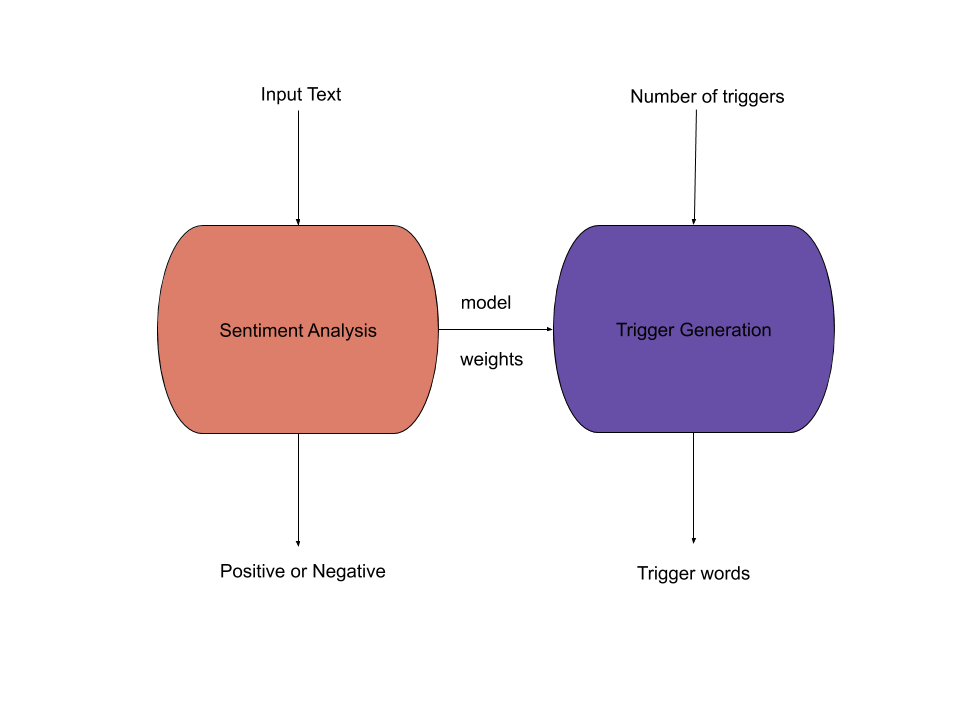
\includegraphics[width=0.8\linewidth]{./img/top_level.png}
  \caption{Top Level Process Flow}
  \label{img: top_level}
\end{figure}


\section{Classifier}
In this project, we train a \textit{Convolutional Neural Network} to classify \textit{Sentiment} of the input text as positive or negative.
 \paragraph{Dataset}
We train our classifier on IMDB dataset \cite{imdb}. It consists of $50,000$ movie reviews from IMBD. It is a binary sentiment classification dataset containing same number of positive and negative reviews. It is constructed only from highly polar review i.e. $\geq$ 7 out of 10 for positive set and $\leq$ 4 out of 10 for negative set. The dataset is evenly divided into training data and testing data consisting of $25000$ movie reviews each.

\paragraph{Pre-Processing}
In order to convert sentence to something suitable for computation, preprocessing is required.
IMBD data contains html tags like line breaker, so first, we remove html tags using python's regex library. We also remove numbers from the moview reviews.
Next, we use spaCy \cite{spacy} to tokenize this sanitized string.
The tokens are then converted to integers using a fixed vocabulary size ($25000$ in our case) and a Vocab lookup table. This is a bidirectional lookup where given a word it outputs its integer value and given integer value its returns its corresponding word.
 
\paragraph{Embeddings}
We use GloVe \cite{glove} word embeddings to represent words as feature vectors.
In particular, we use Glove.6B which has 6 Billion tokens, 400 Thousand uncased vocabulary, and 100 vector dimensions.

\paragraph{Architecture}
We use a CNN to classify senetences. The architecture is referred from \cite{kim2014}.
CNN emulates an n-gram model. Suppose the size of kernel is $3 \times m$, where $m$ is the embedding dimension, then the convolution operation takes $3$ consecutive words together and applies the function over it. Hence, it performs operations on tri-grams of the text.
The architecture of CNN is as shown in the Fig. \ref{img: archi}.

\begin{figure}[!h]
  \centering
  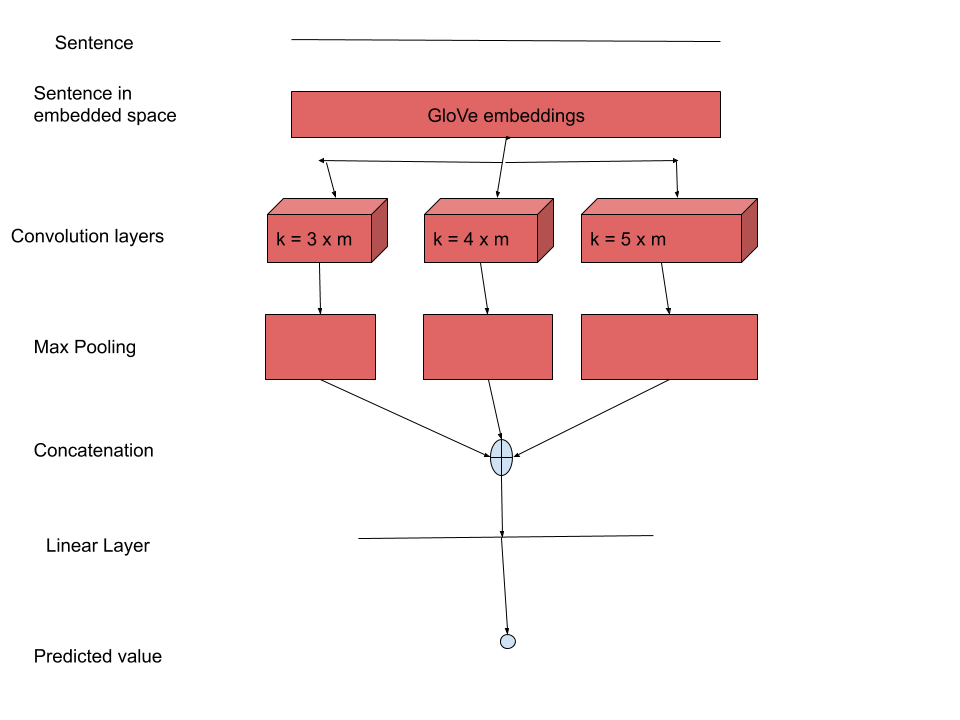
\includegraphics[width=\linewidth]{./img/archi.png}
  \caption{CNN architecture}
  \label{img: archi}
\end{figure}

Our CNN contains 3 filters sizes of $3 \times m$, $4 \times m$, and $5 \times m$, and each size has 100 instances. Hence, we use tri-grams, tetra-grams, and penta-grams of input text to decide its category. 

The output of convolutions are passed through a max pool layer. The idea here is that the feature with maximum value is the critical feature for determining the sentiment of the review.
Then, vectors are concatenated to create a single vector and are passed through Fully Connected Linear(Dense) layer to obtain a single value which corresponds to sentiment of the text.
Continuous value is discretize by passing it through a sigmoid function, and hence, the text is classified into one of the two classes. We use \textit{BCEWithLogitsLoss} loss function implemented in PyTorch \cite{pytorch} as Loss function. It is a Binary Cross Entropy Loss and a Sigmoid layer in one class.

\begin{figure}[ht!]
    \centering
    \begin{subfigure}[t]{0.5\textwidth}
        \centering
        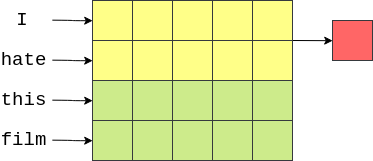
\includegraphics[height=1.2in]{./img/conv_work.png}
        \caption{CNN extracts n-grams}
    \end{subfigure}%
    ~ 
    \begin{subfigure}[t]{0.5\textwidth}
        \centering
        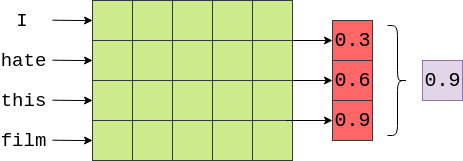
\includegraphics[height=1.2in]{./img/pool_work.png}
        \caption{Max pool}
    \end{subfigure}
    \caption{CNN for sentiment analyis}
 \end{figure}
  
% TODO write about all the hyperparamerters used.
\section{Trigger Generation}
We want to generate trigger words that can attack a targeted class. Ideally, the triggers should be stealthy 
As defined in equation \ref{eq: trigger}, we want to find an advesarial example in which trigger words are prepended to actual sentence. To find the triggers, we optimizer equation \ref{eq: optim}. Since, it is an optimizing problem, it can be given as search algorithm.

\subsection*{Trigger Search Algorithm}
Initially, length of trigger words is chosen. Shorter triggers are more stealthy, while longer triggers are more successful. The words are initialized by the value ``the'', then to optimize the loss function, we iteratively replace trigger tokens over a batch of data. As language is discrete, we use a variant of Hotflip \cite{ebrahimi2018} attack designed by Wallace et al \cite{wallace2019}. Hotflip approximtes the effect of replacing a token using its gradient and embedding space.

\paragraph{Token Replacement Strategy}
This Hotflip based token replacement is based on linaer approximation of the loss function as it converges faster.
The embedding for every trigger token $e_{adv_i}$ is updated to minimizes the loss’ first-order Taylor approximation around the current token embedding:
\begin{equation}
  \label{eq: approx_loss}
  \underset{e_{i}' \in \mathcal{V}}{argmin} \; [e -  e_{adv_i}]^T \; \nabla_{e_{adv_i}} \mathcal{L}
\end{equation}
where, $\mathcal{V}$ is the set of all token embeddings in the model’s vocabulary and $\nabla_{e_{adv_i}} \mathcal{L}$ is the average gradient of the task loss over a batch.
Finnaly, this token $e_{adv_i}$ in embeddeing space is converted to word space. Fig. \ref{trigger_algo} illustrates this algorithm.

\begin{figure}[!h]
  \centering
  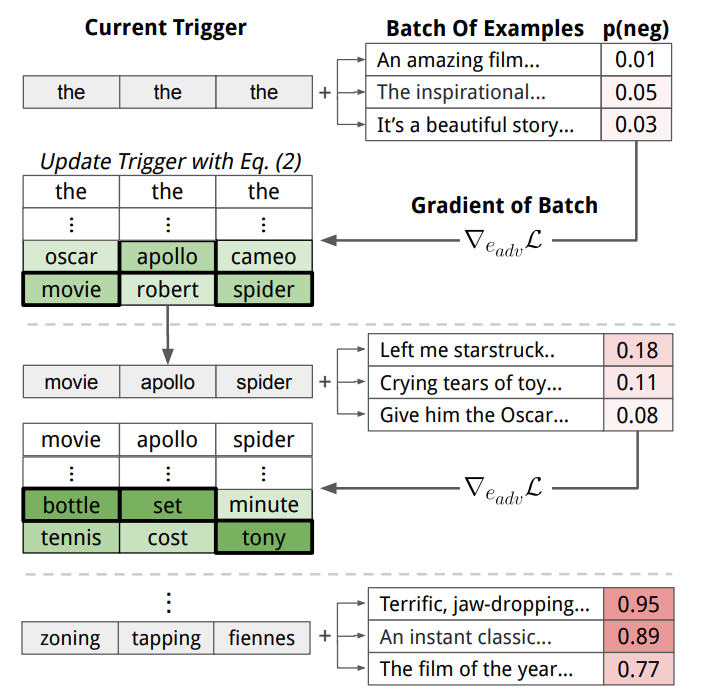
\includegraphics[width=0.8\linewidth]{./img/trigger_algo.png}
  \caption{Trigger Search Algorithm by Wallace et. al. \cite{wallace2019}}
  \label{trigger_algo}
\end{figure}

With the help of beam search, this algorithm is further augmented. Top-$k$ tokens from equation \ref{eq: approx_loss} are considered as candidates to replace current trigger tokens. For every candidate token, its loss with current batch is calculated and one with the optimum loss is chosen. The beam size are constrained as per computation power.

\paragraph{Implementation}
We ``hook'' a pointer on the word embeddings to get its gradients needed to perform trigger search. The gradients obtained for a batch are averaged and only gradients of trigger tokens are passed to \textit{hotflip} function.
\textit{Hotflip} function takes the averaged gradients and word embedding matrix, and extracts top-$k$ candidates from the product of gradients and embeddings. We keep the value of $k = 5$ for computation constraints. With this top canidates, a left to right beam search is carried to obtain new trigger tokens.

\chapter{Output}
\section{Classifier}
Fig. \ref{model_param} shows the parameters and hyper paramters of our model. Number of trainable paramters of outr CNN is $2620801$. Other hyperparamters include learning rate which we kept as $0.001$.

\begin{figure}[!h]
  \centering
  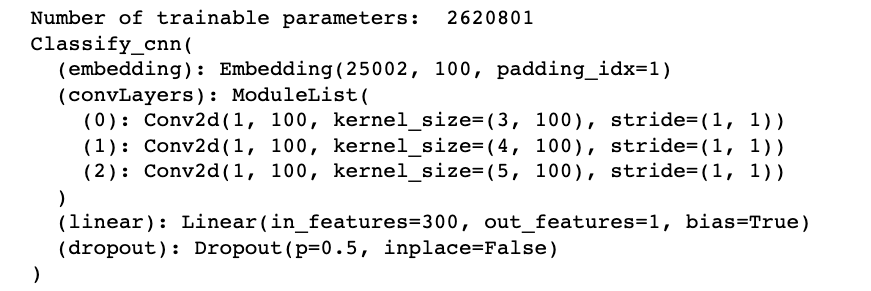
\includegraphics[width=0.6\linewidth]{./img/output/model_param.png}
  \caption{Model parameters and hyperparameters}
  \label{model_param}
\end{figure}

The confusion matrix of the predictions made by our model is shown in Fig. \ref{cm_og}. The number of True positives are $11333$, True Negatives $10654$, False Positive $1167$, and False Negative $1846$. Hence, the accuracy of the model is $87.948\%$

\begin{figure}[ht!]
    \centering
    \begin{subfigure}[t]{0.3\textwidth}
        \centering
        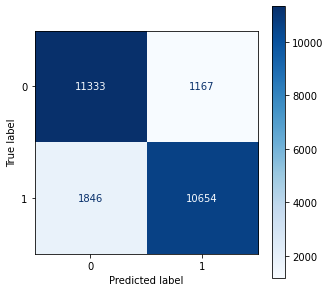
\includegraphics[width=\linewidth]{./img/output/cm_og.png}
        \caption{Confusion matrix of model predictions}
        \label{cm_og}
    \end{subfigure}%
    ~ 
    \begin{subfigure}[t]{0.5\textwidth}
        \centering
        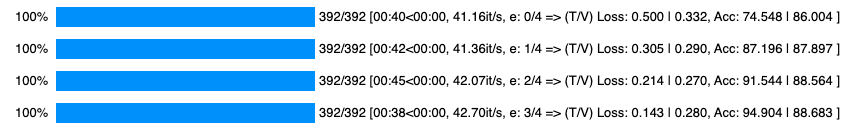
\includegraphics[width=\linewidth]{./img/output/train_loop.png}
        \caption{Train Loop}
    \end{subfigure}
    \caption{Model Training}
 \end{figure}

\section{Trigger Generation}
Fig. \ref{img: trig} shows how the addition of trigger words ``unisol unisol roesnlski'' decrease sensitivity(true positive rate) which implies accuracy of the model also decreases.

\begin{figure}[!h]
  \centering
  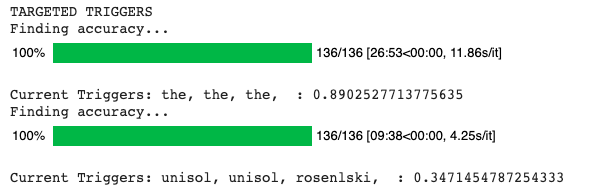
\includegraphics[width=0.8\linewidth]{./img/output/trig.png}
  \caption{Generating Triggers}
  \label{img: trig}
\end{figure}

Some examples demonstrating the effect of Adversarial triggers are shown in Fig. 3.4. These examples point out that our model might be picking up on some biases and noises which leads to oversensitivity to some inputs.

\begin{figure}[h!]
    \label{img: adv_eg}
    \centering
    \begin{subfigure}[t]{\textwidth}
        \centering
        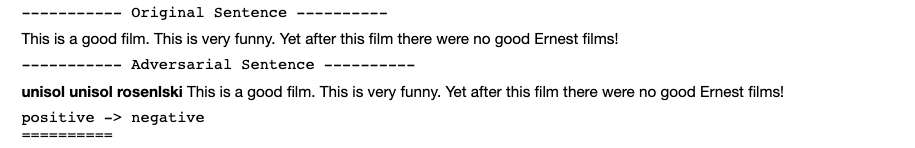
\includegraphics[width=\linewidth]{./img/output/eg_1.png}
        \caption{Eg 1}
        \label{img: eg1}
    \end{subfigure}
    
    \begin{subfigure}[t]{\textwidth}
        \centering
        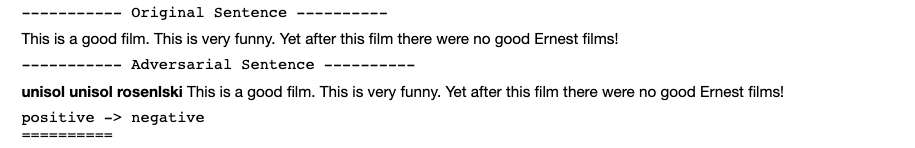
\includegraphics[width=\linewidth]{./img/output/eg_1.png}
        \caption{Eg 2}
        \label{img: eg2}
    \end{subfigure}%

    \begin{subfigure}[t]{\textwidth}
        \centering
        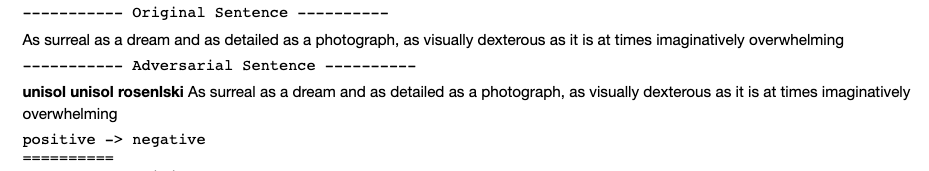
\includegraphics[width=\linewidth]{./img/output/eg_3.png}
        \caption{Eg 3}
        \label{img: eg3}
    \end{subfigure}%

    \begin{subfigure}[t]{\textwidth}
        \centering
        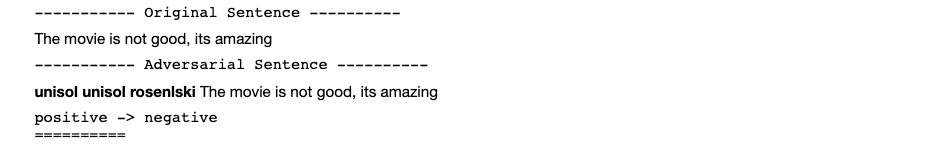
\includegraphics[width=\linewidth]{./img/output/eg_4.png}
        \caption{Eg 4}
        \label{img: eg4}
    \end{subfigure}%

    \caption{Universal Adversarial Trigger examples}
 \end{figure}

\end{spacing}

\renewcommand{\bibname}{References}
\bibliography{report}
\bibliographystyle{ieeetr}

\end{document}
